\documentclass[10pt]{beamer}
\usetheme{Warsaw}

% |===| Package imports.

\usepackage{
  etex, graphicx, amssymb, amsmath, amstext, amsfonts, mathtools,
  multicol, pgfplots, array, listings, colortbl, ulem, ifthen, xcolor
}
\usepackage[scaled=1]{beramono}
\usepackage[T1]{fontenc}
\usepackage[utf8]{inputenc}
\usepackage{tikz}

\usetikzlibrary{shapes,arrows}

\renewcommand{\baselinestretch}{1.2}

% Trying to waste less space

% \addtolength{\topmargin}{1pt}
% \addtolength{\headsep}{5pt}
% \addtolength{\oddsidemargin}{-4pt}
% \addtolength{\marginparwidth}{20pt}
% \addtolength{\marginparsep}{-3pt}
% \addtolength{\textwidth}{-5pt}


% |===| Beamer things.

% |=====| Cyan on black theme.

% |===| Basic colors.
\definecolor{background}{RGB}{0,0,0}
\definecolor{balance}{RGB}{255,255,255}
\definecolor{foreground}{RGB}{102,178,255}

% |===| Other colors.
\definecolor{cstm_red}{RGB}{255,130,130}
\definecolor{cstm_green}{RGB}{130,255,170}
\colorlet{cstm_blue}{foreground}
\definecolor{cstm_orange}{RGB}{255,180,110}
\definecolor{cstm_yellow}{RGB}{255,255,0}

% |===| Special colors.
\colorlet{daiji}{cstm_red}
\colorlet{emph}{balance}
\colorlet{code}{cstm_orange}
\colorlet{url}{balance!80!background}
\colorlet{tikz_neutral}{balance!80!background}

\setbeamercolor{normal text}{
  fg = foreground, bg = background
}
\setbeamercolor{structure}{
  fg = foreground, bg = background
}

\setbeamercolor{alerted text}{
  fg = red!85!background
}

\setbeamercolor{item projected}{
  use = item, fg = background, bg = item.fg!35!balance
}

\setbeamercolor*{palette primary}{
  use = structure, fg = structure.fg
}
\setbeamercolor*{palette secondary}{
  use = structure, fg = structure.fg!95!background
}
\setbeamercolor*{palette tertiary}{
  use = structure, fg = structure.fg!90!background
}
\setbeamercolor*{palette quaternary}{
  use = structure, fg = structure.fg!95!background, bg = background
}

\setbeamercolor*{framesubtitle}{
  fg = background!40
}

\setbeamercolor*{block title}{
  parent = structure, fg = background, bg = cstm_blue!70!balance
}
\setbeamerfont*{block title}{
  series = \bfseries
}
\setbeamercolor*{block body}{
  fg = foreground, bg = background!83!balance
}
\setbeamercolor*{block title alerted}{
  parent = alerted text, bg = background!15!balance
}
\setbeamercolor*{block title example}{
  parent = example text,bg = background!15!balance
}

\setbeamertemplate{navigation symbols}{}
\setbeamertemplate{headline}{}
\setbeamertemplate{frametitle}{
  \large\insertframetitle\hfill\small\insertsection
}
\setbeamertemplate{footline}{}
% \setbeamertemplate{footline}[frame number]{}
% \setbeamerfont{footline}{family = \rmfamily, series = \mdseries, size = \small}
% \setbeamercolor{footline}{ fg = balance }

\setbeamertemplate{itemize item}{\textbullet}


% |===| TOC things.

\AtBeginSection{
  \begin{frame}
  \frametitle{Contents}
  \tiny{\tableofcontents[hideallsubsections, currentsection]}
  \end{frame}
}

\setbeamertemplate{sections/subsections in toc}[circle]
\setbeamerfont{section in toc}{
  size = \large
}
\setbeamerfont{section number projected}{
  series = \bfseries, size = \large
}
\setbeamercolor{section number projected}{
  bg = foreground, fg = background
}

% |===| Tikz things.

% |===| Node styles.

\tikzstyle{empty} = [
  draw=none, fill=none
]

\tikzstyle{rect} = [
  draw=tikz_neutral, ultra thick, font = \bf
]
\tikzstyle{circ} = [
  rect, circle
]
\tikzstyle{elli} = [
  rect, ellipse
]

% |===| Node style modifiers.

\tikzstyle{round} = [
  rounded corners
]

\tikzstyle{drw_red}    = [ draw =    cstm_red ]
\tikzstyle{drw_green}  = [ draw =  cstm_green ]
\tikzstyle{drw_blue}   = [ draw =   cstm_blue ]
\tikzstyle{drw_orange} = [ draw = cstm_orange ]
\tikzstyle{drw_yellow} = [ draw = cstm_yellow ]

\tikzstyle{fil_red}    = [ fill =    cstm_red ]
\tikzstyle{fil_green}  = [ fill =  cstm_green ]
\tikzstyle{fil_blue}   = [ fill =   cstm_blue ]
\tikzstyle{fil_orange} = [ fill = cstm_orange ]
\tikzstyle{fil_yellow} = [ fill = cstm_yellow ]

\tikzstyle{txt_red}    = [ text =    cstm_red ]
\tikzstyle{txt_green}  = [ text =  cstm_green ]
\tikzstyle{txt_blue}   = [ text =   cstm_blue ]
\tikzstyle{txt_orange} = [ text = cstm_orange ]
\tikzstyle{txt_yellow} = [ text = cstm_yellow ]

% |===| Draw styles.

\tikzstyle{line} = [
  rect
]
\tikzstyle{arrow} = [
  rect, ->, >=latex
]

% |===| Macros.

% |===| Formatting.

\newcommand{\daiji}[1]{\textcolor{daiji}{#1}}
\newcommand{\code}[1]{{\small\texttt{\textcolor{code}{#1}}}}
\renewcommand{\emph}[1]{\textit{\textcolor{emph}{#1}}}
\newcommand{\bigsep}{\itemsep1.2em}
\newcommand{\ita}[1]{\textit{#1}}
\newcommand{\prompt}{\code{>}\xspace}
\newcommand{\impl}{\Rightarrow}
\newcommand{\daimpl}{\daiji{$\impl$}\xspace}
\newcommand{\daiheart}{\daiji{$\heartsuit$}\xspace}



% |===| Listings.

\lstdefinelanguage{rust_lst}{
  alsoletter={'},
  % backgroundcolor=\color{white},
  basicstyle = { \scriptsize\ttfamily },
%
% Lifetimes.
%
  keywords=[1]{},
  keywordstyle=[1]\color{cstm_green},
  keywordsprefix=',
%
  morekeywords=[2]{ % Orange
    struct, enum, trait, impl, use, for, while, loop, in, fn, let, pub
  },
  keywordstyle=[2]\color{cstm_orange},
%
  morekeywords=[3]{
    if, then, else, match, =>, ->
  },
  keywordstyle=[3]{\bf\ttfamily\color{foreground!70!yellow}},
%
  morekeywords=[4]{ % Types.
    Self, usize, isize, fsize,
    u8, u16, u32, u64,
    i8, i16, i32, i64,
    f8, f16, f32, f64,
    str, String, Vec, Option, Result,
    \{, \}
  },
  keywordstyle=[4]{\bf\color{balance}},
%
  morekeywords=[5]{
    mut, break, continue, return, !
  },
  keywordstyle=[5]\color{cstm_red},
%
  morekeywords=[6]{
    self
  },
  keywordstyle=[6]\color{balance!90!background},
%
  stringstyle=\color{cstm_yellow},
%
% Macros
%
  literate=*%
    {!}{{\textcolor{cstm_red}{!}}}1
    {\&}{{\textcolor{cstm_green}{\&}}}1
    {->}{{$\to$}}2,
%
% Comments
%
  morecomment=[l]{//},
  morecomment=[n]{/*}{*/},
%
  morecomment=[n][\color{balance!40!background}]{/**}{*/},
  morecomment=[n][\color{balance!40!background}]{/*!}{*/},
  morecomment=[l][\color{balance!40!background}]{///},
  morecomment=[l][\color{balance!40!background}]{//!},
%
  morestring=[b]",
  morestring=[b]""",
  % breakatwhitespace=false,
  % breaklines=true,
  % captionpos=b,
  commentstyle=\color{balance!30!background}\it\bfseries,
  % deletekeywords={...},
  % escapeinside={\%*}{*)},
  % extendedchars=true,
  frame=l,
  % keepspaces=true,
  % keywordstyle=\color{blue},
  % otherkeywords={*,...},
  % numbers=left,
  % numbersep=5pt,
  % numberstyle=\tiny\color{mygray},
  % rulecolor=\color{black},
  sensitive=true,
  % showspaces=false,
  showstringspaces=false,
  % showtabs=false,
  % stepnumber=2,
  % stringstyle=\color{mymauve},
  % tabsize=2
}
\lstnewenvironment{rust}{
  \lstset{ language = rust_lst }
}{
}

% |===| Nice links.

\hypersetup{
  colorlinks=true,
  linkcolor=url,
  urlcolor=url,
  % /!\ REMEMBER TO CHANGE THIS. /!\
  pdftitle={Programming Language Concepts: Intro}
}


% |===| Title page info.

\title{
  Programming Language Concepts\\[3em]
  Introduction\\[2em]
}

\author[]{
  Adrien Champion\\
  \href{mailto:adrien.champion@email.com}{adrien.champion@email.com}
}


\date{}

\begin{document}
\addtolength{\leftmargin}{-20pt}
\addtolength{\rightmargin}{-20pt}



\begin{frame}{}
  \titlepage
\end{frame}



\section{About the class}




\begin{frame}[fragile,t]{Programming languages}

\vspace{4em}

From sources to ``executable''
\medskip

\alt<2->{
  Type system
  \medskip

  \alt<3->{
    Memory management
    \medskip

    \alt<4->{
      Abstraction mechanisms
      \medskip

      \alt<5->{
        Misc.
        \medskip
        \alt<6->{
        }{
          \begin{itemize}
            \item compiler plugins
            \item macros
            \item identation-has-semantics
            \item expressions over statements
          \end{itemize}
        }
      }{
        \begin{itemize}
          \item structures
          \item objects
          \item modules
          \item algebraic data types
          \item type classes (traits)
        \end{itemize}
      }
    }{
      \begin{itemize}
        \item manual
        \item heap / stack
        \item garbage collection
      \end{itemize}
    }
  }{
    \begin{itemize}
      \item none
      \item weak
      \item strong
      \item super-strong
    \end{itemize}
  }
}{
  \begin{itemize}
    \item compile
    \item interpret
  \end{itemize}
}

\end{frame}




\begin{frame}{Guidelines}

Software:
\medskip
\begin{itemize}
  \item (private) version control (\daiji{bitbucket} or \daiji{github})
  \item \daiji{Rust} compiler (\code{rustc}) and project manager (\code{cargo})
  \item unix-based system recommended (\daiji{VM} on Windows)
\end{itemize}
\bigskip

\pause

Resources for Rust:\\
\medskip
\begin{tabular}{r l}
  official & \url{https://www.rust-lang.org/} \\
  online compiler & \url{https://play.rust-lang.org/} \\
  tutorial & \url{https://doc.rust-lang.org/stable/book/} \\
  & \url{http://rustbyexample.com/} \\
  API & \url{https://doc.rust-lang.org/stable/std/} \\
  libraries & \url{https://crates.io/} \\
\end{tabular}

\end{frame}





\begin{frame}{Assignments / Projects}

\begin{itemize}
  \bigsep
  \item you \daiji{can} discuss ideas / algorithms
  \item you \daiji{\bf CANNOT} share code
  \item I \daiji{will not} deal with cheating, the university will
\end{itemize}
\bigskip

\pause

Assignments in \daiji{Rust}:

\begin{itemize}
  \item \emph{$2048$}
\end{itemize}

\end{frame}





\begin{frame}{Roadmap}

\[
  \begin{array}{r l}
    \left.
    \begin{aligned}
      \text{Abstract machines}\\
      \text{Describing a language}\\
      \text{Foundations}\\
      \text{Memory management}\\
    \end{aligned}
    \uncover<2->{\quad\right\rbrace} &
    \uncover<2->{
      \text{
        \begin{tabular}{c}
          theory and \daiji{runtime}
        \end{tabular}
      }
    } \\\\
    \uncover<3->{
      \left.
      \begin{aligned}
        \text{Names and environment}\\
        \text{Control structures}\\
        \text{Control abstraction}\\
        \text{Structuring data}\\
        \text{Data abstraction}\\
      \end{aligned}
    }
    \uncover<4->{\quad\right\rbrace} &
    \uncover<4->{
      \text{
        \begin{tabular}{c}
          abstractions, control flow, and\\
          from \daiji{source} to \daiji{target}
        \end{tabular}
      }
    }
  \end{array}
\]

\end{frame}





\begin{frame}{Your experience}

Which languages have you used or just know about?
\bigskip

What about them?
\medskip
\begin{itemize}
  \item in which context are they typically used? (web, software, \ldots)
  \item compiled or interpreted?
  \item memory management?
  \item type system?
  \item abstraction mechanisms?
\end{itemize}

\end{frame}






\section{Rust}



\begin{frame}{Memory management}
  \emph{Life cycle} of memory is always the same:
  \smallskip
  \begin{itemize}
    \item \daiji{allocate} memory you need
    \item \daiji{use} it (read / write)
    \item \daiji{free} the memory when it is not used anymore
  \end{itemize}
  \medskip

  Generally speaking,
  \begin{itemize}
    \item \daiji{allocation} is manual, happens when declaring a variable
    \item \daiji{using} memory is manual: actual code
  \end{itemize}
\end{frame}



\begin{frame}{Memory management}
  \daiji{Freeing} memory is a challenge, in mainstream languages it can be
  \begin{itemize}
    \item \emph{manual}: \code{malloc} / \code{free}\\
      \hfill C (\emph{1970}), C++\\
      very old-skool
    \item \emph{automatic} at runtime: garbage collection\\
      \hfill Java (\emph{1995}), C\#, JavaScript, Python, F\#, OCaml, \ldots\\
      \pause
      Actually invented in \daiji{1959} for the Lisp language\\
      pretty old-skool too
  \end{itemize}
\end{frame}




\begin{frame}{Memory management}
  \emph{Garbage collection} (GC):
  \begin{itemize}
    \item \daiji{easy} to use, because transparent to the developer
    \item memory is \emph{automagically} freed when ``not used anymore''
    \item<2-> \daiji{problem}: \emph{magic} is expensive in CS
  \end{itemize}
  \bigskip\uncover<3->{
    \emph{Manual memory management}:
    \begin{itemize}
      \item \daiji{no overhead}, developer frees memory manually\\
      \item<4-> but very complex and thus \daiji{error-prone} (memory leaks)
      \item<4-> \daiji{Nightmare} for concurrent programs sharing data
    \end{itemize}
  }
  \bigskip
  \uncover<5->{
    In general developers \daiji{$\heartsuit$} garbage collection:\\
    mindless, and fast hardware hides the overhead anyway\ldots
  }
\end{frame}




\begin{frame}{Problem solved?}
  \emph{GC} shows its limits when doing \daiji{expensive computations},\\
  with a lot of allocation
  \bigskip

  \begin{itemize}
    \item \daiji{HPC} \hfill (High Performance Calculus, applied maths),
    \item solving problems with \daiji{exponential complexity},
    \item \daiji{web browsers} \hfill (surprisingly expensive),
    \item \ldots
  \end{itemize}
\end{frame}




\begin{frame}{Rust}

Why Rust?

\begin{center}
  \url{http://www.cnet.com/news/samsung-joins-mozillas-quest-for-rust/}
\end{center}

\bigskip

\begin{tabular}{r l | r}
\pause $\bullet$ &
  memory / thread \daiji{safety} &
  strong typing, ownership,\\
& &
  regional memory management\\\hline

\pause $\bullet$ &
  powerful \daiji{abstractions} &
  first-class functions, type classes\\\hline

\pause $\bullet$ &
  \daiji{defensive} approach &
  \code{Result} / \code{Option} instead of\\
& &
   exceptions and \code{null}\\\hline

\pause $\bullet$ &
  \daiji{performance} &
  compiles to LLVM,\\
& &
  no garbage collection\\
\end{tabular}

% \bigskip
% \pause

% Goals:

% \begin{itemize}
% \item safety and security
% \item maintainability
% \item extensibility
% \end{itemize}

\end{frame}




\begin{frame}{Rust, in short}

  \begin{itemize}
    \item \daiji{safety} and \daiji{performance} first
    \item support for \daiji{concurrency}
    \item hi-level \daiji{abstractions}
    \item avoid error-prone \daiji{paradigms}
  \end{itemize}

\end{frame}


% \begin{frame}[fragile]{\daiji{$2048$}: data abstraction}

% \begin{minipage}[t]{.5\textwidth}

% \daiji{Structs}
% \medskip

% \lstset{language = rust_lst}
% \begin{lstlisting}
% /// Power of two in a cell.
% pub struct Cell {
%   pow: u32,
% }
% \end{lstlisting}

% Gather data in a single structure

% \end{minipage}%
% %
% ~%
% %
% \begin{minipage}[t]{.5\textwidth}

% \daiji{Enums}
% \medskip

% \lstset{language = rust_lst}
% \begin{lstlisting}
% /// *Swipe* directions.
% pub enum Dir {
%   Up, Dw, Lf, Rg,
% }
% \end{lstlisting}

% Alternatives of what the value can be

% \end{minipage}

% \end{frame}






% \begin{frame}[fragile]{Malloc / free (intuition)}

% \begin{minipage}[t]{.39\textwidth}
% \begin{rust}
% let res = {
%   let lhs = 42 ;
%   let rhs = 7  ;
%   lhs + rhs
% } ;
% \end{rust}
% \medskip
% What happens at runtime?
% \end{minipage}~\begin{minipage}[t]{.60\textwidth}
% \pause
% \begin{rust}
% let ref_res = malloc(64) ;
% let ref_lhs = malloc(64) ; * ref_lhs = 42 ;
% let ref_rhs = malloc(64) ; * ref_rhs = 7  ;
% * ref_res = * ref_lhs + * ref_rhs ;
% free(ref_lhs) ; free(ref_rhs)
% \end{rust}
% \end{minipage}

% \bigskip
% \pause

% \begin{center}
%   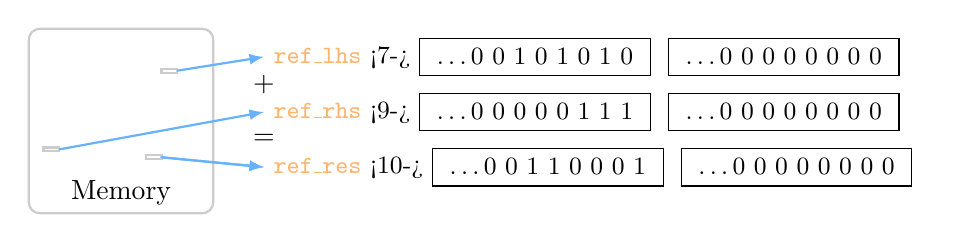
\begin{tikzpicture}

\def\blkW{0.2}
\def\blkH{0.05}

\def\resX{1.7}
\def\resY{1.8}

\def\lhsX{0.2}
\def\lhsY{0.8}

\def\rhsX{1.5}
\def\rhsY{0.7}

\def\keyX{3}
\def\keyY{2}
\def\keySep{0.7}

% Memory.
\node[
  rect, round, anchor = south west, thick,
  text width = 6em, text height = 6em
] (memory) at (0,0) {} ;
\node[
  empty, anchor = south
] () at (memory.south) {Memory} ;

% `res`.
\uncover<4->{
  \draw[
    rect, thick
  ] (\rhsX,         \rhsY        ) --
    (\rhsX,         \rhsY + \blkH) --
    (\rhsX + \blkW, \rhsY + \blkH) --
    (\rhsX + \blkW, \rhsY        ) --
    cycle
  ;
}
\uncover<5->{
  \node[empty, anchor = west] (refRes) at (\keyX, \keyY - 2 * \keySep) {
    \small
    \code{ref\_res}
    \alt<10->{
      \begin{tabular}{|c|}
        \hline\ldots 0 0 1 1 0 0 0 1\\\hline
      \end{tabular}
    }{
      \begin{tabular}{|c|}
        \hline\ldots 0 0 0 0 0 0 0 0\\\hline
      \end{tabular}
    }
  } ;
}
\uncover<5>{
  \draw[arrow, thick, drw_blue] (
    \rhsX + \blkW, \rhsY + 0.5 * \blkH
  ) -- (refRes.west) ;
}
\uncover<10>{
  \draw[arrow, thick, drw_blue] (
    \rhsX + \blkW, \rhsY + 0.5 * \blkH
  ) -- (refRes.west) ;
}

% `lhs`.
\uncover<6-10>{
  \draw[
    rect, thick
  ] (\resX,         \resY        ) --
    (\resX,         \resY + \blkH) --
    (\resX + \blkW, \resY + \blkH) --
    (\resX + \blkW, \resY        ) --
    cycle
  ;
  \node[empty, anchor = west] (refLhs) at (\keyX, \keyY) {
    \small
    \code{ref\_lhs}
    \alt<7->{
      \begin{tabular}{|c|}
        \hline\ldots 0 0 1 0 1 0 1 0\\\hline
      \end{tabular}
    }{
      \begin{tabular}{|c|}
        \hline\ldots 0 0 0 0 0 0 0 0\\\hline
      \end{tabular}
    }
  } ;
}
\uncover<6-7>{
  \draw[arrow, thick, drw_blue] (
    \resX + \blkW, \resY + 0.5 * \blkH
  ) -- (refLhs.west) ;
}

\uncover<10>{
  \node[empty] () at (\keyX, \keyY - 0.5*\keySep) {$+$} ;
}

% `rhs`.
\uncover<12>{}
\uncover<8-11>{
  \draw[
    rect, thick
  ] (\lhsX,         \lhsY        ) --
    (\lhsX,         \lhsY + \blkH) --
    (\lhsX + \blkW, \lhsY + \blkH) --
    (\lhsX + \blkW, \lhsY        ) --
    cycle
  ;
  \node[empty, anchor = west] (refRhs) at (\keyX, \keyY - \keySep) {
    \small
    \code{ref\_rhs}
    \alt<9->{
      \begin{tabular}{|c|}
        \hline\ldots 0 0 0 0 0 1 1 1\\\hline
      \end{tabular}
    }{
      \begin{tabular}{|c|}
        \hline\ldots 0 0 0 0 0 0 0 0\\\hline
      \end{tabular}
    }
  } ;
}
\uncover<8-9>{
  \draw[arrow, thick, drw_blue] (
    \lhsX + \blkW, \lhsY + 0.5 * \blkH
  ) -- (refRhs.west) ;
}

\uncover<10>{
  \node[empty] () at (\keyX, \keyY - 1.5*\keySep) {$=$} ;
}

\end{tikzpicture}
% \end{center}

% \end{frame}






% \begin{frame}[fragile]{Garbage collection (intuition)}

% \begin{minipage}[t]{.39\textwidth}
% \begin{rust}
% let res = {
%   let lhs = 42 ;
%   let rhs = 7  ;
%   lhs + rhs
% } ;
% \end{rust}
% \medskip
% What happens at runtime?
% \end{minipage}~\begin{minipage}[t]{.60\textwidth}
% \pause
% \begin{rust}
% let ref_res = malloc(64) ;
% let ref_lhs = malloc(64) ; * ref_lhs = 42 ;
% let ref_rhs = malloc(64) ; * ref_rhs = 7  ;
% * ref_res = * ref_lhs + * ref_rhs ;
% free(ref_lhs) ; free(ref_rhs)
% \end{rust}
% \end{minipage}

% \end{frame}







% \section{Test frames}



% \begin{frame}{Block example}

%   \begin{block}{Block's title}
%     This is the content of the block.
%   \end{block}

% \end{frame}




% \begin{frame}[fragile]{Rust example}

% \lstset{language = rust_lst}
% \begin{lstlisting}
% /// A trait.
% pub trait MyTrait {
%   fn mk() -> Self ;
%   fn set(& mut self, usize) ;
% }

% /** A structure. */
% pub struct MyStruct {
%   field: usize
% }
% // Implementation of the structure.
% impl MyStruct {
%   /// Public constructor.
%   pub fn of(n: usize) -> Self {
%     MyStruct { field: n } /* This is how you create a structure. */
%   }
%   pub fn to_str(&self, pref: & 'static str) -> String {
%     format!("{}{}", pref, self.field)
%   }
% }
% impl MyTrait for MyStruct {
%   fn mk() -> Self { self.of(0) }
%   fn set(& mut self, n: usize) { self.field = n }
% }
% \end{lstlisting}

% \end{frame}






% \begin{frame}{Tikz example}

%   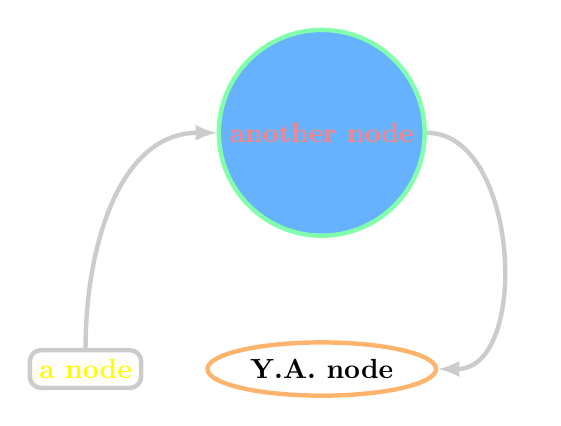
\begin{tikzpicture}

\node[rect, round, txt_yellow] (n1) at (0,0) { a node } ;
\node[circ, drw_green, fil_blue, txt_red] (n2) at (3,3) { another node } ;
\node[elli, drw_orange] (n3) at (3,0) { Y.A. node } ;

\draw[arrow] (n1) to[out=90, in=180] (n2) ;
\draw[arrow] (n2) to[out=0, in=0] (n3) ;

\end{tikzpicture}


% \end{frame}





\end{document}
